\documentclass[twoside, letterpaper, 12pt]{report}
\usepackage{orthodoxservicebook}

\title{The Sunday Reader's Service of the \\ \textsc{Typica} \\  2020 March 29}
\titlepic{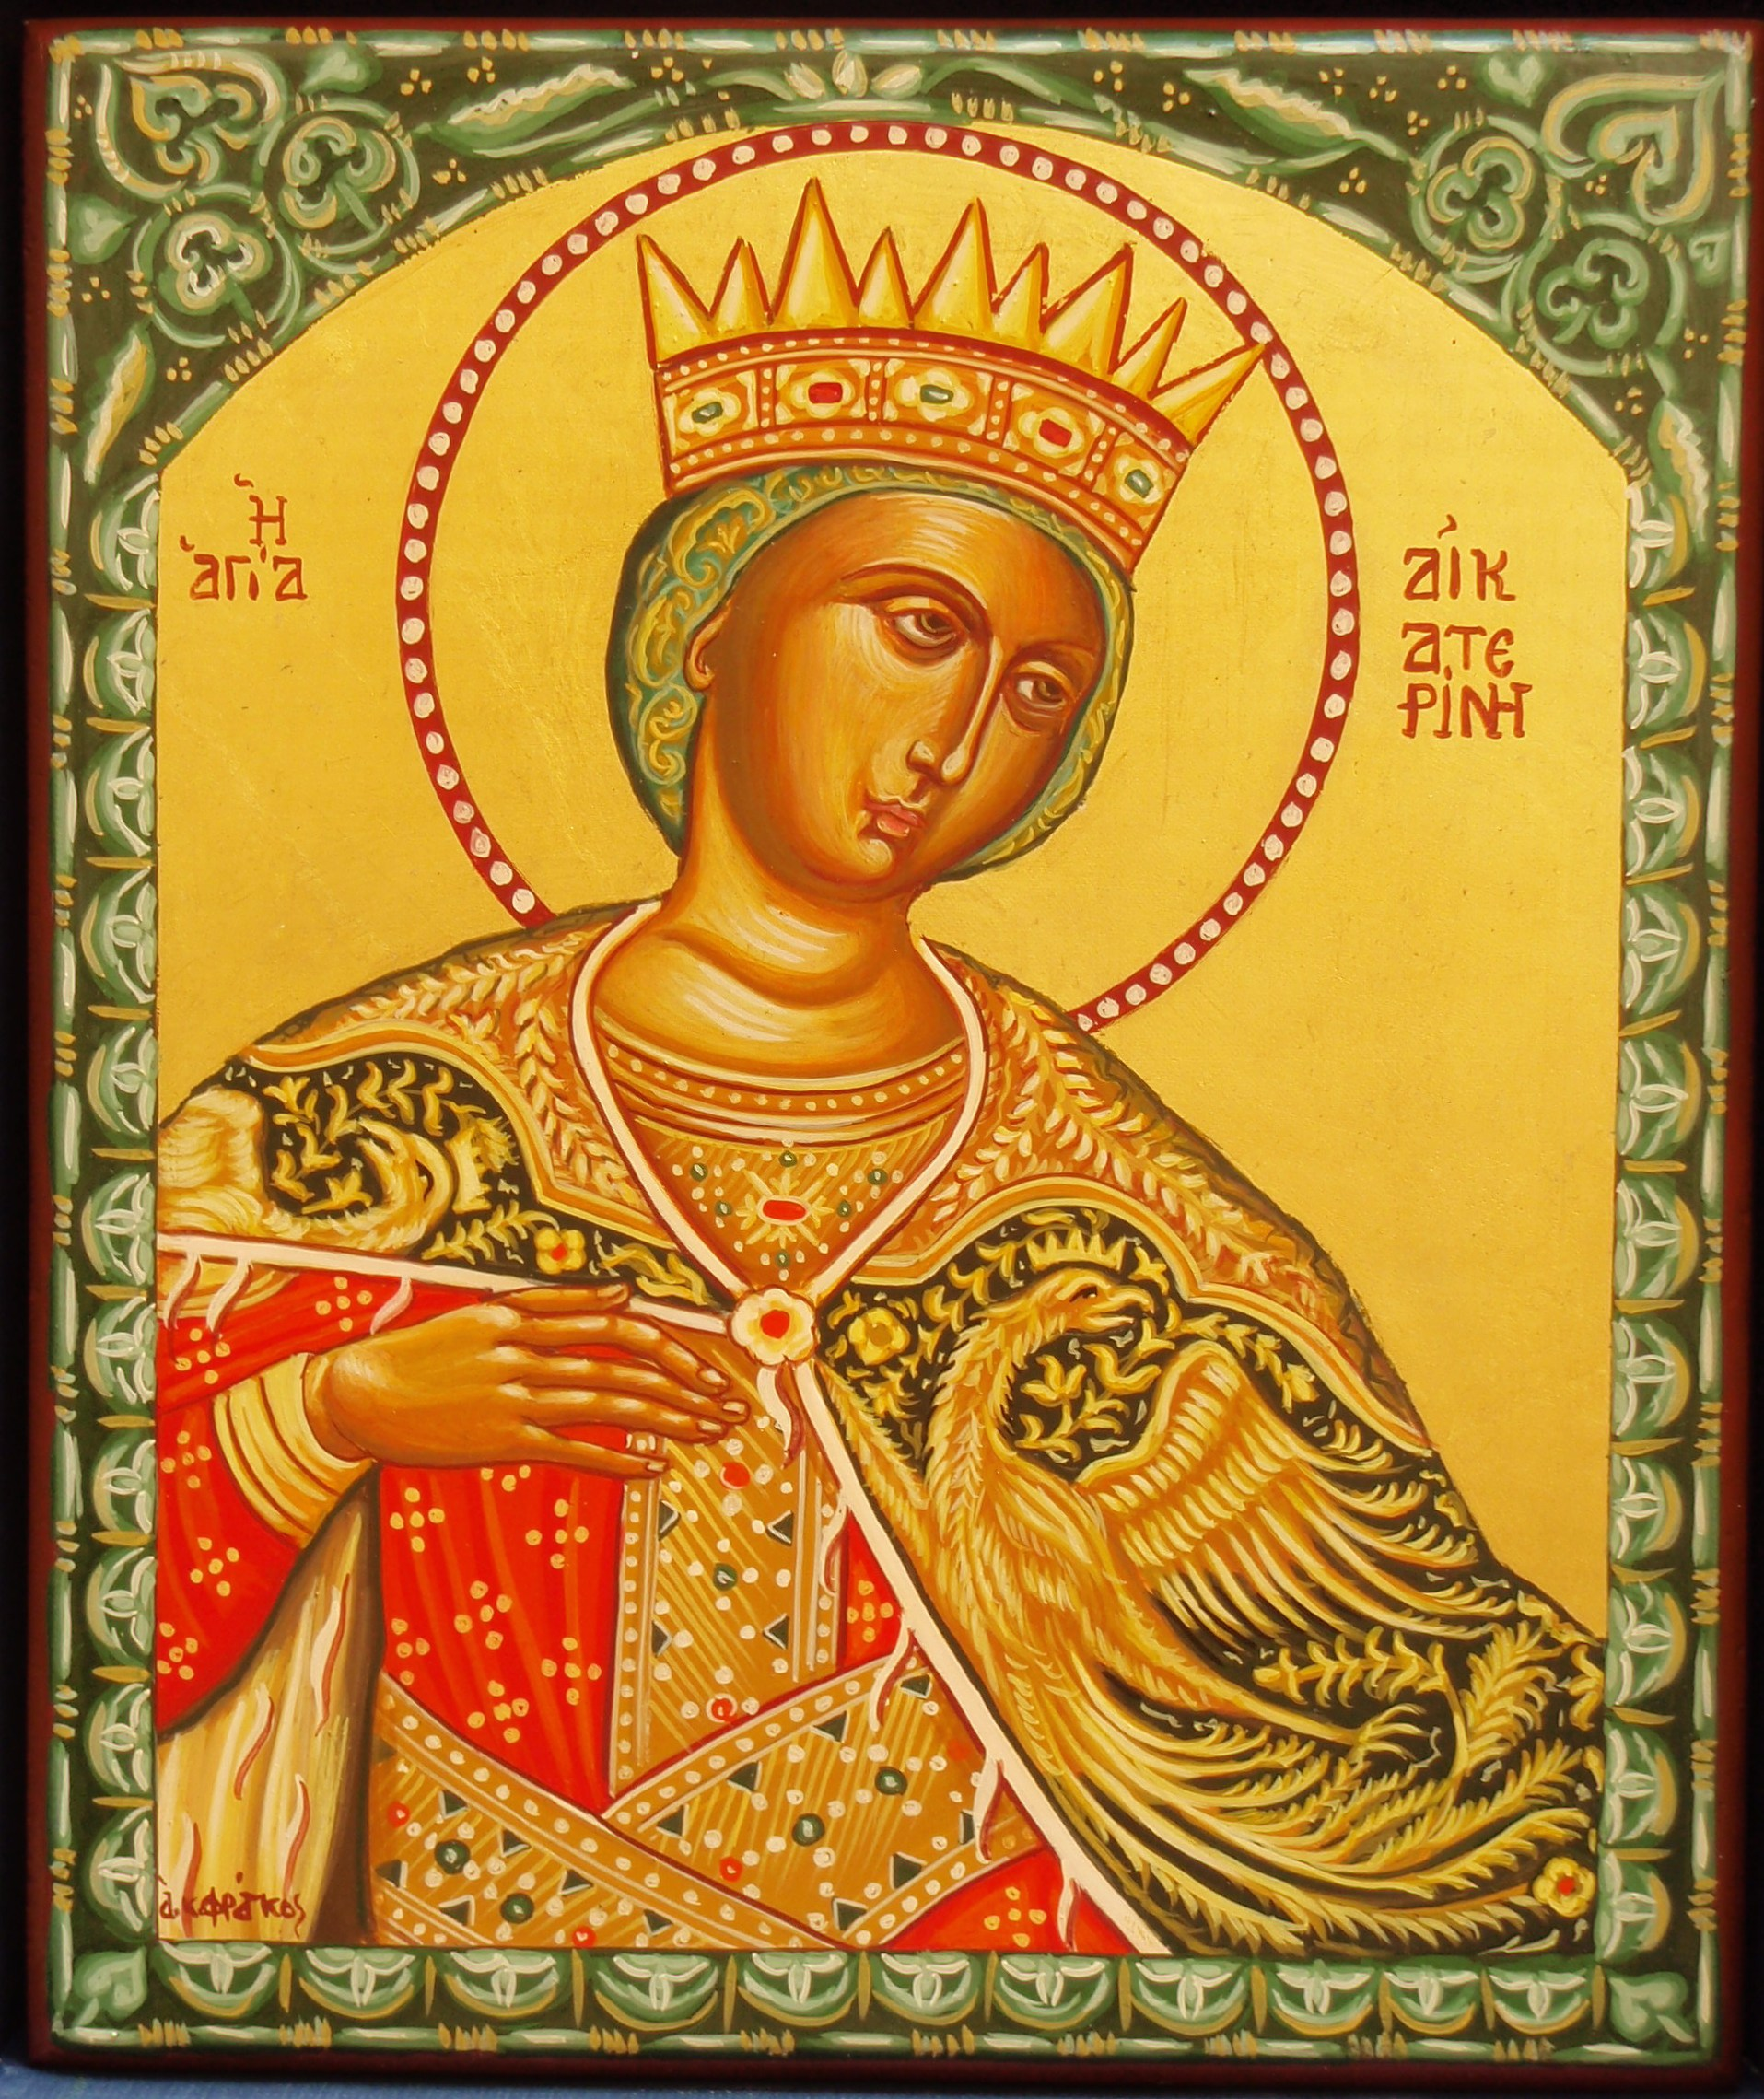
\includegraphics[width=0.5\textwidth]{Katherine1.jpg}}
\date{}
\author{}

\begin{document}
\maketitle
\pagestyle{empty} % Don't show page numbers
\instruction{This page intentionally left blank}
\cleardoublepage
\pagestyle{plain}
\setcounter{page}{1} % Set the page counter to 1 on the first real page
\chapter*{The Sunday Reader's Service of Typica\\ 2020 March 29}
\readerline{Through the prayers of our holy fathers, Lord Jesus Christ our God,
  have mercy on us, and save us}
\lilypondfile{./Z-Responses/Obikhod/Amen.ly}

\trisagionNeedsAmen[reader]
\lilypondfile{./Z-Responses/Obikhod/Amen.ly}


\centeredsection{The First Antiphon}
\lilypondfile{./Liturgy/B-FirstAntiphon/BlessTheLord_Greek-Music.ly}

\centeredsection{The Second Antiphon}
\lilypondfile{./Liturgy/C-SecondAntiphon/PraiseTheLord_Greek-Music.ly}

\centeredsection{The Third Antiphon}
\lilypondfile{./Liturgy/D-ThirdAntiphon/Beatitudes_Moscow-Music.ly}

\centeredsection{The Epistle}

\instruction{Both of the New Testament lessons are read
without liturgical introduction or conclusion.
The readers start with “The Reading from…” and proceeds}

\paragraph{The Reading from the Epistle of St. Paul to the Hebrews. (6:13-20)}\mbox{}\\

Brethren, when God made a promise to Abraham, since He had no one greater by whom
to swear, He swore by Himself, saying, “Surely I will bless you and multiply you.” And thus
Abraham, having patiently endured, obtained the promise. Men indeed swear by one greater than
themselves, and in all their disputes an oath is final for confirmation. So when God desired to show
more convincingly to the heirs of the promise the unchangeable character of His purpose, He
interposed with an oath. So that through two unchangeable things, in which it is impossible that
God should prove false, we who have fled for refuge might have strong encouragement to seize
the hope set before us. We have this as a sure and steadfast anchor of the soul, a hope that enters
into the inner shrine behind the curtain, where Jesus has gone as a forerunner on our behalf, having
become a high priest forever after the order of Melchizedek.

\centeredsection{The Gospel}

\instruction{Both of the New Testament lessons are read
without liturgical introduction or conclusion.
The readers start with “The Reading from…” and proceeds}

\paragraph{The Reading from the Holy Gospel according to St. Mark. (9:17-31)}\mbox{}\\

At that time, a man came to Jesus, kneeling down and saying unto him, “Teacher, I brought
my son to you, for he has a dumb spirit. And wherever it seizes him, it dashes him down; and he
foams and grinds his teeth and becomes rigid; and I asked Thy Disciples to cast it out, and they
were not able.” And Jesus answered them, “O faithless generation, how long am I to be with you?
How long am I to bear with you? Bring him to Me.” And they brought the boy to Him; and when
the spirit saw Jesus, immediately it convulsed the boy, and he fell on the ground and rolled about,
foaming at the mouth. And Jesus asked his father, “How long has he had this?” And he said, “From
childhood. And it has often cast him into the fire and into the water, to destroy him; but if Thou
canst do anything, have pity on us and help us.” And Jesus said to him, “If you can believe, all
things are possible to him who believes.” Immediately the father of the child cried out and said
with tears, “Lord, I believe; help my unbelief!” And when Jesus saw that a crowd came running
together, he rebuked the unclean spirit, saying to it, “You dumb and deaf spirit, I command you,
come out of him, and never enter him again.” And after crying out and convulsing him terribly, it
came out, and the boy was like a corpse; so that most of them said, “He is dead.” But Jesus took
him by the hand and lifted him up, and he arose. And when Jesus had entered the house, His
Disciples asked Him privately, “Why could we not cast it out?” And Jesus said to them, “This kind
cannot be driven out by anything but prayer and fasting.” They went on from there and passed
through Galilee. And Jesus would not have anyone know it; for He was teaching His Disciples,
saying to them, “The Son of man will be delivered into the hands of men, and they will kill Him;
and after He is killed, He will rise on the third day.”


\centeredsection{Troparia Before the Creed}
\instruction{Plain reading}
\begin{reader}
\item[Reader 1:] The heavenly choir singeth thy praises, saying:
  Holy, holy, holy, Lord of Sabaoth; heaven and earth are full of Thy glory.

\item[Reader 2:] \emph{Come unto him, and be enlightened,
               and your faces shall not be ashamed.}
  The heavenly choir singeth thy praises, saying:
  Holy, holy, holy, Lord of Sabaoth; heaven and earth are full of Thy glory.

\item[Reader 1:] \emph{\glory}
  The choir of the holy angels and archangels,
  with all the powers of heaven, singeth thy praises, saying:
  Holy, holy, holy, Lord of Sabaoth; heaven and earth are full of Thy glory.

\item[Reader 2:]\emph{\nowandever}
\end{reader}

\centeredsection{The Creed}
\input{Common/TheCreed.txt}


\centeredsection{Prayer of Forgiveness}
\readerline{Forgive, remit, pardon, O God, our sins,
  both voluntary and involuntary, in deed and in word, in knowledge or in ignorance,
  committed by night or by day, in mind and in thought.
  Forgive us them all, for thou art good and lovest mankind.
}


\centeredsection{The Lord’s Prayer}
\input{Common/LordsPrayer.txt}

\readerline{Through the prayers of our holy fathers, Lord Jesus Christ our God, have mercy on us.}
\lilypondfile{./Z-Responses/Obikhod/Amen.ly}


\centeredsection{Kontakia for Sundays in Great Lent}
\lilypondfile{./Menaion/03-25-AnnunciationOfTheTheotokos/AnnunciationOfTheTheotokos-Kontakion-T8-Essey-Music.ly}


\readerline{\lhmForty}

\readerline{
  O Christ our God, Who art worshipped and glorified at all times at every hour both in
  heaven and on earth; Who art long-suffering and plenteous in mercy and compassion; Who lovest
  the just man and showest mercy upon the sinner; and Who callest all men to repentance through 
  the promise of blessings to come; receive, O Lord, at this very hour our supplications, and direct
  our lives in the way of Thy commandments: sanctify our souls, purify our bodies, set our minds
  aright, cleanse our thoughts; deliver us from all affliction, trouble, and distress; compass us about
  with Thy holy angels, that, guided and guarded by them, we may attain unto the unity of the Faith,
  and to the knowledge of Thine unapproachable glory; for Thou art blessed unto ages of ages. Amen.
}

\begin{reader}
  \item \lhmThree{}\\\emph{\gne{}}
  \item \morehonorablethanthetherubim{}
  \item \throughtheprayers{}
\end{reader}

\begin{maybetwocolumns}
\lilypondfile{./Z-Responses/Obikhod/Amen.ly}

\readerline{\blessedbethename{}\thrice{}}

\centeredsection{Psalm 33}
\input{./Psalms/Psalm033-unknowntrans.txt}

\centeredsection{Psalm 144}
\input{./Psalms/Psalm144-unknowntrans.txt}
\end{maybetwocolumns}

\peopleline{\gne}


\centeredsection{A Homily}
\begin{maybetwocolumns}
\instruction{Father George Aquaro - 4th Sunday of lent, second Sunday of Quarantine}

In the Name of the Father, and of the Son, and of the Holy Spirit!

Today, the fourth Sunday of Great Lent, finds us locked away in our homes.
In a way, this is not unlike the ancient Lenten practice of isolation during the 40 days of fasting.

We find ourselves cut off from others, avoiding direct contact,
and trying to deal with the rigors of 'less.' In the isolation,
or perhaps decrease in distractions and stimulation,
we suddenly discover how dependent we are on so many things of this world.

In the liturgy, we sing, “Let us lay aside all earthly care,
that we may receive the King of All...” Spiritual growth is about laying aside earthly cares.
In order to 'climb the ladder' of spiritual development,
we have to leave the concerns of the ground where the ladder begins,
so that we can concentrate on the next rung.
It does not mean we are 'carefree' in the sense that nothing bothers or concerns us at all,
but that our concerns are in keeping with our ascent to God.

If we are concerned with other people and what they do or think,
are we really thinking about God and getting closer to Him? No, we are not.
On the ladder of spiritual ascent, one climbs alone.
It is Christ Himself who is the ladder, because He bears us to His Father.
And, while the choirs of the angels and saints may cheer us on, they do not climb for us.
Each of us must climb on his own, which is why no two Christians have identical spiritual journeys.

No one else can make you climb, nor force you off.
Remember, Christ is the ladder, and no man is more powerful than God.
However, if we become distracted,
if we watch the wind as St. Peter did when Jesus beckoned him to walk with Him on the water,
we will sink as did the Apostle.
We ought not be distracted by other people or the storms of circumstances,
both those present and those imagined to come.

We have no control over this world, and our Lord admonishes us to not pay too much attention to it.
Just like a real ladder, if you lose focus on what you're doing, you may slip.
In such instances, it is not that the ladder lets go of you, but you let go of the ladder.

And, if you are heavy laden with many cares, the ladder takes greater effort to climb,
and you are more likely to fall. This is why, as we climb,
we often find ourselves shedding unwanted things that become to heavy to carry.

I remember as a boy going on a backpacking trip,
and having a large frame pack filled with enough gear to survive a month in the woods.
We were going out for a three day trek.
At first, it felt good to be prepared for any eventuality,
until I hit mile ten and realized there was still two and a half days of hiking left
and my body was at its limits.
The other adults went through my bag, split up the items that weighed me down,
and helped me survive the rest of journey.
It was a less in being over-prepared, and how there is such a thing as 'too much.'

Some things are helpful, others are not
What is helpful in one circumstance is not helpful in another.
Having a -20° sleeping bag isn't necessary when you are on a summer hike.
Sure, you may get lost,
but the chance of that bag saving your life is about as remote as winning the lottery.
Of course, you can carry it.
The trick is to not grumble that your pack is too full and too heavy.

You make the choices of what you can try to carry up the ladder,
but the experiences of the Holy Fathers teach us that the higher you go, the more you leave behind.
Your pride. Your expectations. Your desires for things. Your requirements for others to follow.
Those things get heavy along the way even if you somehow leave the ground with them.

The greatest danger that faces the spiritual climber is the delusion that you are climbing when you
really aren't. This is an easy trap to fall into.
We assume that the weight of all our cares IS the strain of our ascetic development,
when it is not.
We think that because we are sweating under the enormous burden of our cares that we are somehow
more spiritual precisely because we care so much.

Caring is not a virtue. Everyone has cares, even if those cares are about avoiding cares.
Even caring for others can quickly devolve into codependency and mental illness.
The quantity or quality of your cares does not make them appropriate.
Finding out what cares are helpful and which are not requires spiritual guidance from others.

As we continue on this journey towards Pascha,
we can genuinely say that we do not know what lies ahead.
Will we be permitted to return to the mission to serve Christ,
or will we be having our Paschal celebrations at home under continued 'mini-quarantine'?
I don't think anyone knows for sure, and worrying about it does not help.

Jesus Christ is our ladder, and we climb this ladder no matter where we are.
Shed the worries and cares, for the journey is life-long.
Some things aren't worth taking to the very end.
Let go of the burdens, lay aside the cares,
and take the next step up towards your Heavenly Father.

\end{maybetwocolumns}

\centeredsection{Resurrectional Apolytikion in Tone 8}
\lilypondfile{./Octoechos/ResurrectionalApolytikion-Tone8-Kazan-Music.ly}

\centeredsection{Apolytikion of St. John Climacus in Tone 8}

The barren wilderness thou didst make fertile with the streams of thy tears; and by thy deep sighing
thou hast given fruit through thy struggles a hundredfold. Accordingly, thou hast become a star for
the universe, sparkling with miracles. Therefore, O righteous Father John Climacus, intercede with
Christ God to save our souls.

\readerline{\throughtheprayers}

\lilypondfile{./Z-Responses/Obikhod/Amen.ly}

\end{document}

